\documentclass[twocolumn]{aa}

\usepackage{graphicx}
\usepackage{amsmath,amsfonts,amssymb}
\usepackage{txfonts}
\usepackage{color}
%\usepackage{fixltx2e}
\usepackage{natbib}
%\usepackage{caption,subcaption}
%\usepackage{epsfig}
\usepackage{float}
%\usepackage{stfloats}
\usepackage{dblfloatfix}
\usepackage{afterpage}
\usepackage{ifthen}
\usepackage[morefloats=12]{morefloats}
\usepackage{placeins}
\usepackage{multicol}
%\usepackage[breaklinks,colorlinks,citecolor=blue]{hyperref}
\bibpunct{(}{)}{;}{a}{}{,}
\usepackage[switch]{lineno}
\definecolor{linkcolor}{rgb}{0.6,0,0}
\definecolor{citecolor}{rgb}{0,0,0.75}
\definecolor{urlcolor}{rgb}{0.12,0.46,0.7}
\usepackage[breaklinks, colorlinks, urlcolor=urlcolor,
    linkcolor=linkcolor,citecolor=citecolor,pdfencoding=auto]{hyperref}
\hypersetup{linktocpage}
\usepackage{bold-extra}
\usepackage{xcolor}
\usepackage{tabularx}
\usepackage{csquotes}
\usepackage{breakurl}
\usepackage{lipsum}
\usepackage{mathtools}
\usepackage{cuted}
\usepackage{upgreek}


%Planck style file, to be used with A&A style to produce Planck papers for publication.
%
% version 28 September 2010 --- useful macros --- CRL
% version 17 October 2010   --- first cut at important instrument values, from Daniele Mennella and
%                               Francois Bouchet, 13 October 2010 --- CRL
% version 18 October 2010   --- LFI FWHM changed to one value per feed, rather than M & S separately
%                               LFI FWHM uncertainties added for individual feeds.  Corrections made
%                               to LFI values. --- Andrea Zacchei
% version 24 October 2010   --- added to and corrected definitions.  No changes made to instrument
%                               quantities. --- CRL 
% version 31 October 2010   --- added definition of \muKHz. --- CRL
%
% version 15 November 2010  --- fixed conflict with aa.cls in definition of \endtable
%                               by naming the command below "\endPlancktable".  See section
%                               13.16 of the Style Guide.
%
% version 06 December 2010  --- Set up names with and without units.
%                               Add \allearlypapers command to ensure that all early papers are
%                               included in the reference list.
%                               Define macro for the name of the 4He JT cooler.
%
% version 07 December 2010  --- removed extraneous "planck2011-1.2" entry in \allearlypapers
%
% version 12 December 2010  --- added \endPlancktablewide command to set tablenotes to the full
%                               page width in the \begin{table*}...\end{table*} environment when
%                               the ``twocolumn'' option is specified in the \documentclass command.
%                               (It would be more elegant to extract the appropriate width from the
%                               aa.cls system at the time of execution, but that is buried more
%                               deeply in the system than I investigated.)
%
% version 05 January 2011   --- added unit \MJysr.  HFI performance values updated per FRB email
%                               01/05/2011 02:38-0800, and Brendan Crill email 01/05/2011 18:08 -0800.
%
% version 06 January 2011   --- changed \scriptscriptstyle primes to \scriptstyle, to better match the
%                               tx fonts used by A&A.
%
% version 07 January 2011   --- modified \allearlypapers to correspond with final early paper list.  
%                               Fixed 545 GHz center frequency.
%
% version 07 January 2011b  --- changed LFI white-noise sensitivity numbers to correct problem with units
%
% version 05 July 2011      --- added \Msol and \Lsol to get the symbols for solar mass and luminosity.
%                               Deleted previous definitions of \solar and \sol, which were equivalent
%                               to the new \Msol.
%
% version 16 August 2011    --- changed comments on \endPlancktable and \endPlancktablewide for clarity
%
% version 11 September 2011 --- changed definition of \tablenote to make footnote labels italic, as per A\&A
%
% version 26 April 2011     --- changed definition of \Planck to agree with what is said in the Style Guide (!)
%
% version 04 Dec 2013       --- included 2013 results references
%
% version 17 Jan 2014       --- included fix to bibtex file v4.3, i.e. \providecommand{\sorthelp}[1]{}
%
% version 26 Jul 2014       --- fixed incompatibility problem with aa.cls v8.0 and v8.2.  v8.2 should now be used
%                               for all Planck papers.
%                           --- fixed problem in definition of "\all2013resultspapers" that introduced a blanck
%                               into the reference to p06b.
%                           --- removed all the parameter definition stuff at the end.  We weren't using it, and
%                               it took up a lot of space.
%
% version 28 Jan 2015       --- added "\alltwentyfiftennresultspapers" and corrected "\all2013resultspapers" to
%                               "\all20thirteenresultspapers",
%
% Usage:  after the \documentclass[traditabstract]{aa} command in the La\TeX\ input file,
%         add this command:      \input Planck.tex


\def\setsymbol#1#2{\expandafter\def\csname #1\endcsname{#2}}
\def\getsymbol#1{\csname #1\endcsname}

%-----------------------------------------------------------------------
% Planck
%-----------------------------------------------------------------------
\def\Planck{\textit{Planck}}

%-----------------------------------------------------------------------
% The Planck Helium-4 JT cooler
%-----------------------------------------------------------------------
\def\HeJT{$^4$He-JT}

%-----------------------------------------------------------------------
% To include all Planck Early Results papers in the reference lists
%-----------------------------------------------------------------------
\def\allearlypapers{\nocite{planck2011-1.1, planck2011-1.3, planck2011-1.4, planck2011-1.5, planck2011-1.6, planck2011-1.7, planck2011-1.10, planck2011-1.10sup, planck2011-5.1a, planck2011-5.1b, planck2011-5.2a, planck2011-5.2b, planck2011-5.2c, planck2011-6.1, planck2011-6.2, planck2011-6.3a, planck2011-6.4a, planck2011-6.4b, planck2011-6.6, planck2011-7.0, planck2011-7.2, planck2011-7.3, planck2011-7.7a, planck2011-7.7b, planck2011-7.12, planck2011-7.13}}

%-----------------------------------------------------------------------
% To include all Planck 2013 Results papers in the reference lists
%-----------------------------------------------------------------------
\def\alltwentythirteenresultspapers{\nocite{planck2013-p01, planck2013-p02, planck2013-p02a, planck2013-p02d, planck2013-p02b, planck2013-p03, planck2013-p03c, planck2013-p03f, planck2013-p03d, planck2013-p03e, planck2013-p01a, planck2013-p06, planck2013-p03a, planck2013-pip88, planck2013-p08, planck2013-p11, planck2013-p12, planck2013-p13, planck2013-p14, planck2013-p15, planck2013-p05b, planck2013-p17, planck2013-p09, planck2013-p09a, planck2013-p20, planck2013-p19, planck2013-pipaberration, planck2013-p05, planck2013-p05a, planck2013-pip56, planck2013-p06b, planck2013-p01a}}

%-----------------------------------------------------------------------
% To include all Planck 2015 Results papers in the reference lists
%-----------------------------------------------------------------------
\def\alltwentyfifteenresultspapers{\nocite{planck2014-a01, planck2014-a03, planck2014-a04, planck2014-a05, planck2014-a06, planck2014-a07, planck2014-a08, planck2014-a09, planck2014-a11, planck2014-a12, planck2014-a13, planck2014-a14, planck2014-a15, planck2014-a16, planck2014-a17, planck2014-a18, planck2014-a19, planck2014-a20, planck2014-a22, planck2014-a24, planck2014-a26, planck2014-a28, planck2014-a29, planck2014-a30, planck2014-a31, planck2014-a35, planck2014-a36, planck2014-a37, planck2014-ES}}

%-----------------------------------------------------------------------
% Tables
%-----------------------------------------------------------------------
\newbox\tablebox    \newdimen\tablewidth
\def\leaderfil{\leaders\hbox to 5pt{\hss.\hss}\hfil}
%
% use the following definition of \endPlancktable for ApJ style notes to tables, set to the 
%         width of the table
% \def\endPlancktable{\tablewidth=\wd\tablebox 
%
% use the following definitions of \endPlancktable and \endPlancktablewide for A&A style notes 
% set to one-column  or full-page width, respectively
\def\endPlancktable{\tablewidth=\columnwidth 
    $$\hss\copy\tablebox\hss$$
    \vskip-\lastskip\vskip -2pt}
\def\endPlancktablewide{\tablewidth=\textwidth 
    $$\hss\copy\tablebox\hss$$
    \vskip-\lastskip\vskip -2pt}
\def\tablenote#1 #2\par{\begingroup \parindent=0.8em
    \abovedisplayshortskip=0pt\belowdisplayshortskip=0pt
    \noindent
    $$\hss\vbox{\hsize\tablewidth \hangindent=\parindent \hangafter=1 \noindent
    \hbox to \parindent{$^#1$\hss}\strut#2\strut\par}\hss$$
    \endgroup}
\def\doubleline{\vskip 3pt\hrule \vskip 1.5pt \hrule \vskip 5pt}

%-----------------------------------------------------------------------
% useful macros
%-----------------------------------------------------------------------
%
\def\L2{\ifmmode L_2\else $L_2$\fi}
%
\def\dtt{\Delta T/T}
\def\DeltaT{\ifmmode \Delta T\else $\Delta T$\fi}
\def\deltat{\ifmmode \Delta t\else $\Delta t$\fi}
\def\fknee{\ifmmode f_{\rm knee}\else $f_{\rm knee}$\fi}
\def\Fmax{\ifmmode F_{\rm max}\else $F_{\rm max}$\fi}
%
\def\solar{\ifmmode{\rm M}_{\mathord\odot}\else${\rm M}_{\mathord\odot}$\fi}
\def\Msolar{\ifmmode{\rm M}_{\mathord\odot}\else${\rm M}_{\mathord\odot}$\fi}
\def\Lsolar{\ifmmode{\rm L}_{\mathord\odot}\else${\rm L}_{\mathord\odot}$\fi}
%
\def\inv{\ifmmode^{-1}\else$^{-1}$\fi}
\def\mo{\ifmmode^{-1}\else$^{-1}$\fi}
\def\sup#1{\ifmmode ^{\rm #1}\else $^{\rm #1}$\fi}
\def\expo#1{\ifmmode \times 10^{#1}\else $\times 10^{#1}$\fi}
%
\def\,{\thinspace}
\def\lsim{\mathrel{\raise .4ex\hbox{\rlap{$<$}\lower 1.2ex\hbox{$\sim$}}}}
\def\gsim{\mathrel{\raise .4ex\hbox{\rlap{$>$}\lower 1.2ex\hbox{$\sim$}}}}
\let\lea=\lsim
\let\gea=\gsim
\def\simprop{\mathrel{\raise .4ex\hbox{\rlap{$\propto$}\lower 1.2ex\hbox{$\sim$}}}}
%
\def\deg{\ifmmode^\circ\else$^\circ$\fi}
\def\pdeg{\ifmmode $\setbox0=\hbox{$^{\circ}$}\rlap{\hskip.11\wd0 .}$^{\circ}
          \else \setbox0=\hbox{$^{\circ}$}\rlap{\hskip.11\wd0 .}$^{\circ}$\fi}
\def\arcs{\ifmmode {^{\scriptstyle\prime\prime}}
          \else $^{\scriptstyle\prime\prime}$\fi}
\def\arcm{\ifmmode {^{\scriptstyle\prime}}
          \else $^{\scriptstyle\prime}$\fi}
\newdimen\sa  \newdimen\sb
\def\parcs{\sa=.07em \sb=.03em
     \ifmmode \hbox{\rlap{.}}^{\scriptstyle\prime\kern -\sb\prime}\hbox{\kern -\sa}
     \else \rlap{.}$^{\scriptstyle\prime\kern -\sb\prime}$\kern -\sa\fi}
\def\parcm{\sa=.08em \sb=.03em
     \ifmmode \hbox{\rlap{.}\kern\sa}^{\scriptstyle\prime}\hbox{\kern-\sb}
     \else \rlap{.}\kern\sa$^{\scriptstyle\prime}$\kern-\sb\fi}
%
\def\ra[#1 #2 #3.#4]{#1\sup{h}#2\sup{m}#3\sup{s}\llap.#4}
\def\dec[#1 #2 #3.#4]{#1\deg#2\arcm#3\arcs\llap.#4}
\def\deco[#1 #2 #3]{#1\deg#2\arcm#3\arcs}
\def\rra[#1 #2]{#1\sup{h}#2\sup{m}}
%
\def\page{\vfill\eject}
\def\dots{\relax\ifmmode \ldots\else $\ldots$\fi}
%
%-----------------------------------------------------------------------
% units
%-----------------------------------------------------------------------
%
\def\WHzsr{\ifmmode $W\,Hz\mo\,sr\mo$\else W\,Hz\mo\,sr\mo\fi}
\def\mHz{\ifmmode $\,mHz$\else \,mHz\fi}
\def\GHz{\ifmmode $\,GHz$\else \,GHz\fi}
\def\mKs{\ifmmode $\,mK\,s$^{1/2}\else \,mK\,s$^{1/2}$\fi}
\def\muKs{\ifmmode \,\mu$K\,s$^{1/2}\else \,$\mu$K\,s$^{1/2}$\fi}
\def\muKRJs{\ifmmode \,\mu$K$_{\rm RJ}$\,s$^{1/2}\else \,$\mu$K$_{\rm RJ}$\,s$^{1/2}$\fi}
\def\muKHz{\ifmmode \,\mu$K\,Hz$^{-1/2}\else \,$\mu$K\,Hz$^{-1/2}$\fi}
\def\MJysr{\ifmmode \,$MJy\,sr\mo$\else \,MJy\,sr\mo\fi}
\def\MJysrmK{\ifmmode \,$MJy\,sr\mo$\,mK$_{\rm CMB}\mo\else \,MJy\,sr\mo\,mK$_{\rm CMB}\mo$\fi}
\def\microns{\ifmmode \,\mu$m$\else \,$\mu$m\fi}
\def\micron{\microns}
\def\muK{\ifmmode \,\mu$K$\else \,$\mu$\hbox{K}\fi}
\def\microK{\ifmmode \,\mu$K$\else \,$\mu$\hbox{K}\fi}
\def\muW{\ifmmode \,\mu$W$\else \,$\mu$\hbox{W}\fi}
\def\kms{\ifmmode $\,km\,s$^{-1}\else \,km\,s$^{-1}$\fi}
\def\kmsMpc{\ifmmode $\,\kms\,Mpc\mo$\else \,\kms\,Mpc\mo\fi}
%
%
%----------------------------------------------------------------------
% set up machinery to list Planck papers in roman numeral order.
%----------------------------------------------------------------------

\providecommand{\sorthelp}[1]{}

\def\WMAP{WMAP}
\def\COBE{COBE}
\def\LCDM{$\Lambda$CDM}
\def\ffp{FFP6}
\def\unionmask{U73}
\def\nside{N_{\mathrm{side}}}

\def\healpix{\texttt{HEALPix}}
\def\commander{\texttt{Commander}}
\def\commanderone{\texttt{Commander1}}
\def\commandertwo{\texttt{Commander2}}
\def\commanderthree{\texttt{Commander3}}
\def\ruler{\texttt{Ruler}}
\def\comrul{\texttt{Commander-Ruler}}
\def\CR{\texttt{C-R}}
\def\nilc{\texttt{NILC}}
\def\gnilc{\texttt{GNILC}}
\def\sevem{\texttt{SEVEM}}
\def\smica{\texttt{SMICA}}
\def\CamSpec{\texttt{CamSpec}}
\def\Plik{\texttt{Plik}}
\def\XFaster{\texttt{XFaster}}

\renewcommand{\d}[0]{\vec{d}}
\renewcommand{\t}[0]{\vec{t}}
\newcommand{\A}[0]{\tens{A}}
%\newcommand{\Y}[0]{\tens{Y}}
\newcommand{\Y}[0]{\tens{Y}}
\newcommand{\n}[0]{\vec{n}}
\newcommand{\red}[0]{\color{red}}
\newcommand{\green}[0]{\color{green}}
\newcommand{\s}[0]{\vec{s}}
\renewcommand{\a}[0]{\vec{a}}
\newcommand{\m}[0]{\vec{m}}
\newcommand{\f}[0]{\vec{f}}
\newcommand{\F}[0]{\tens{F}}
\newcommand{\B}[0]{\tens{B}}
\newcommand{\T}[0]{\tens{T}}
\newcommand{\Cp}[0]{\tens{C}}
\renewcommand{\L}[0]{\tens{L}}
\newcommand{\g}[0]{\vec{g}}
\newcommand{\N}[0]{\tens{N}}
\newcommand{\M}[0]{\tens{M}}
\newcommand{\iN}[0]{\tens{N}^{-1}}
\newcommand{\iM}[0]{\tens{M}^{-1}}
\newcommand{\w}[0]{\vec{w}}
\renewcommand{\S}[0]{\tens{S}}
\renewcommand{\r}[0]{\vec{r}}
\renewcommand{\u}[0]{\vec{u}}
\newcommand{\q}[0]{\vec{q}}
\renewcommand{\v}[0]{\vec{v}}
\renewcommand{\P}[0]{\tens{P}}
\newcommand{\dt}[0]{d_t}
\newcommand{\di}[0]{d_i}
\newcommand{\nt}[0]{n_t}
\newcommand{\st}[0]{s_t}
\newcommand{\mt}[0]{m_t}
\newcommand{\ft}[0]{f_t}
\newcommand{\Te}[0]{T_{\rm e}}
\newcommand{\EM}[0]{\rm EM}
\newcommand{\mathsc}[1]{{\normalfont\textsc{#1}}}
\newcommand{\hi}{\ensuremath{\mathsc {Hi}}}
\newcommand{\bpbold}{\bfseries{\scshape{BeyondPlanck}}}
\newcommand{\BP}{\textsc{BeyondPlanck}}
\newcommand{\lfi}[0]{LFI}
\newcommand{\hfi}[0]{HFI}
\newcommand{\npipe}[0]{\texttt{NPIPE}}


\def\bC{\tens{C}}
\def\ba{\vec{a}}
\def\ncha{N_\mathrm{cha}}
\def\nfg{N_\mathrm{fg}}

%\modulolinenumbers[5]
%\linenumbers

\newcommand{\includegraphicsdpi}[3]{
    \pdfimageresolution=#1  % Change the dpi of images
    \includegraphics[#2]{#3}
    \pdfimageresolution=72  % Change it back to the default
}

\renewcommand{\topfraction}{1.0}	% max fraction of floats at top
    \renewcommand{\bottomfraction}{1.0}	% max fraction of floats at bottom
    %   Parameters for TEXT pages (not float pages):
    \setcounter{topnumber}{2}
    \setcounter{bottomnumber}{2}
    \setcounter{totalnumber}{4}     % 2 may work better
    \setcounter{dbltopnumber}{2}    % for 2-column pages
    \renewcommand{\dbltopfraction}{0.9}	% fit big float above 2-col. text
    \renewcommand{\textfraction}{0.04}	% allow minimal text w. figs
    %   Parameters for FLOAT pages (not text pages):
    \renewcommand{\floatpagefraction}{0.9}	% require fuller float pages
	% N.B.: floatpagefraction MUST be less than topfraction !!
    \renewcommand{\dblfloatpagefraction}{0.9}	% require fuller float pages

\def\adj{^{\dagger}}
\def\tp{^{\rm T}}
\def\inv{^{-1}}
\def\lm{{\ell m}}

\begin{document}

\title{\bfseries{\scshape{BeyondPlanck}} XVI. Application to simulated LiteBIRD observations}
%This author list corresponds to \title{Author list for L04\_CMB\_Foregrounds\_Extraction}
%Prepared by M. Lopez-Caniego (Marcos.Lopez.Caniego@sciops.esa.int), ESAC/ESA
%This version is from Thu Jul 12 18:11:48 2018 CET
%\subtitle{There are 152 co-authors in this list}
\newcommand{\nersc}[0]{1}
\newcommand{\princeton}[0]{2}
\newcommand{\helsinkiA}[0]{3}
\newcommand{\milanoA}[0]{4}
\newcommand{\triesteA}[0]{5}
\newcommand{\haverford}[0]{6}
\newcommand{\helsinkiB}[0]{7}
\newcommand{\triesteB}[0]{8}
\newcommand{\milanoB}[0]{9}
\newcommand{\milanoC}[0]{10}
\newcommand{\oslo}[0]{11}
\newcommand{\jpl}[0]{12}
\newcommand{\mpa}[0]{13}
\newcommand{\planetek}[0]{14}
\author{\small
R.~Aurlien\inst{\oslo}\thanks{Corresponding author: R.~Aurlien; \url{ragnhild.aurlien@astro.uio.no}}:
\textcolor{black}{R.~Banerji}\inst{\oslo}
\and
K.~J.~Andersen\inst{\oslo}
\and
M.~Bersanelli\inst{\milanoA, \milanoB, \milanoC}
\and
S.~Bertocco\inst{\triesteB}
\and
M.~Brilenkov\inst{\oslo}
\and
M.~Carbone\inst{\planetek}
\and
L.~P.~L.~Colombo\inst{\milanoA}
\and
H.~K.~Eriksen\inst{\oslo}
\and
\textcolor{black}{M.~K.~Foss}\inst{\oslo}
\and
C.~Franceschet\inst{\milanoA, \milanoC}
\and
\textcolor{black}{U.~Fuskeland}\inst{\oslo}
\and
S.~Galeotta\inst{\triesteB}
\and
M.~Galloway\inst{\oslo}
\and
S.~Gerakakis\inst{\planetek}
\and
E.~Gjerl{\o}w\inst{\oslo}
\and
\textcolor{black}{B.~Hensley}\inst{\princeton}
\and
\textcolor{black}{D.~Herman}\inst{\oslo}
\and
M.~Iacobellis\inst{\planetek}
\and
M.~Ieronymaki\inst{\planetek}
\and
\textcolor{black}{H.~T.~Ihle}\inst{\oslo}
\and
J.~B.~Jewell\inst{\jpl}
\and
\textcolor{black}{A.~Karakci}\inst{\oslo}
\and
E.~Keih\"{a}nen\inst{\helsinkiA, \helsinkiB}
\and
R.~Keskitalo\inst{\nersc}
\and
G.~Maggio\inst{\triesteB}
\and
D.~Maino\inst{\milanoA, \milanoB, \milanoC}
\and
M.~Maris\inst{\triesteB}
\and
S.~Paradiso\inst{\milanoA,\milanoC}
\and
M.~Reinecke\inst{\mpa}
\and
A.-S.~Suur-Uski\inst{\helsinkiA, \helsinkiB}
\and
T.~L.~Svalheim\inst{\oslo}
\and
D.~Tavagnacco\inst{\triesteB, \triesteA}
\and
H.~Thommesen\inst{\oslo}
\and
D.~J.~Watts\inst{\oslo}
\and
I.~K.~Wehus\inst{\oslo}
\and
A.~Zacchei\inst{\triesteB}
}
\institute{\small
Computational Cosmology Center, Lawrence Berkeley National Laboratory, Berkeley, California, U.S.A.\goodbreak
\and
Department of Astrophysical Sciences, Princeton University, Princeton, NJ 08544,
U.S.A.\goodbreak
\and
Department of Physics, Gustaf H\"{a}llstr\"{o}min katu 2, University of Helsinki, Helsinki, Finland\goodbreak
\and
Dipartimento di Fisica, Universit\`{a} degli Studi di Milano, Via Celoria, 16, Milano, Italy\goodbreak
\and
Dipartimento di Fisica, Universit\`{a} degli Studi di Trieste, via A. Valerio 2, Trieste, Italy\goodbreak
\and
Haverford College Astronomy Department, 370 Lancaster Avenue,
Haverford, Pennsylvania, U.S.A.\goodbreak
\and
Helsinki Institute of Physics, Gustaf H\"{a}llstr\"{o}min katu 2, University of Helsinki, Helsinki, Finland\goodbreak
\and
INAF - Osservatorio Astronomico di Trieste, Via G.B. Tiepolo 11, Trieste, Italy\goodbreak
\and
INAF/IASF Milano, Via E. Bassini 15, Milano, Italy\goodbreak
\and
INFN, Sezione di Milano, Via Celoria 16, Milano, Italy\goodbreak
\and
Institute of Theoretical Astrophysics, University of Oslo, Blindern, Oslo, Norway\goodbreak
\and
Jet Propulsion Laboratory, California Institute of Technology, 4800 Oak Grove Drive, Pasadena, California, U.S.A.\goodbreak
\and
Max-Planck-Institut f\"{u}r Astrophysik, Karl-Schwarzschild-Str. 1, 85741 Garching, Germany\goodbreak
\and
Planetek Hellas, Leoforos Kifisias 44, Marousi 151 25, Greece\goodbreak
}

\authorrunning{BeyondPlanck Collaboration}
\titlerunning{Overview}

% Abstract: 1) The first sentence should state what the paper is about. It is often easy to start with the word "We...", as in "We present..." or  "We review.." or "We describe...". 2) The next few sentences should give the context of the paper, and would typically involve both the scientific problem in question and how it fits in. For many papers, the word "BeyondPlanck" will be included here. 3) Next you state what is new in this paper. 4) Then you summarize the main results; remember to include numerical results whenever appropriate. 5) Next, list open problems or the path forward, if relevant. 6) If appropriate, end with a positive sentence of some type.

\abstract{We demonstrate how the {\scshape{BeyondPlanck}} pipeline can be used on 
simulated observations from JAXAs LiteBIRD experiment. LiteBIRD is a full sky cosmic microwave background (CMB) experiment due to be launched in the late 2020s with the scientific goal to detect B-mode from inflationary gravitational waves. 
The {\scshape{BeyondPlanck}} pipeline perform complete integrated end-to-end Bayesian analysis on simulated CMB time ordered data. The analysis shows that the {\scshape{BeyondPlanck}} pipeline is able to reproduce the input data within an uncertainty of ... }

\keywords{ISM: general -- Cosmology: observations, polarization,
    cosmic microwave background, diffuse radiation -- Galaxy:
    general}

\maketitle

% Mathematical symbols in italic. CMB or other words in roman \rm{CMB} (Remove math?)
% Never start caption with "the", "this shows" etc. 
% Galactic with capitol G if referring to Milkyway
% No white space around figures. Change with width=\
% Do not use png, is pixelized. Use pdf or 
% Fig.~6 if in text (check)
% \citeal - ingen parentes, hvis hele teksten skrives i parentes
% \citep - i parentes
% \citet  - årstall i parentes
%\citep[See e.g][and references therin] havner også i parentesen
% rotate y axis labels 90 degrees, align/parallell with axes. Minimizes white space
% Size of text in Figures the same size as text

%\hypersetup{linkcolor=black}
%\tableofcontents
%\hypersetup{linkcolor=red} 


\section{Introduction}
\label{sec:introduction}
%1) The first paragraphs should define the context of the paper: What is the big picture, and why is it important. 2) The next paragraphs should then describe the current state-of-the-art: What has other people done? Include enough references here. 3) Next you describe what the main open problems are. 4) Then you describe what this paper is about and does, and how it improves on the current state-of-the-art. 5) Finally, you may round off with a "table of contents", stating what each of the next section do.

%Storyline intro: Big Bang has been highly successful. Predicted CMB (what the CMB is). Found in 1965. After that three space missions. Next piece of puzzle: gravitational waves from inflation. B-mode. Difficult to detect, in need of extreme precision. BP and joint sampling to help with this. Demonstrate possible in this paper.

% Section on the CMB
The leading theory describing the creation of the universe is the highly successful Big Bang Theory. The missing piece within  this theory yet to be detected is signals from the period of cosmic inflation. It is theorised that the universe expanded exponentially in this first fraction of a nanosecond after its birth, creating ripples in spacetime called gravitational waves. These ripples would have created curl patterns in the polarized Cosmic Microwave Background (CMB), the so called B-mode. Detecting these is the next big goal in cosmology and pushes the required instruments and sensitivities to the extreme. 

%would explain why the univers is highly homogeneous. 

% Section on status today, overview of fullsky experiments and introducing LiteBIRD

The CMB radiation was released 380.000 years after the Big Bang started, in the period of recombination. At that time, the CMB photons had a temperature of 3000~K. Today, after 13.8~Billion years of expansion of the universe, this radiation has cooled down to 2.7255~K \citep{fixsen2009} and was first detected in the microwave regime in 1965 by \citet{penzias:1965}. After the first detection there have been several CMB experiments, three of these have been full sky space missions. The latest state-of-the-art mission was the Planck space mission launched in 2009 \citep{planck2016-l01}, following up on the Cosmic Background Explorer (COBE) from 1989 (\citealp{mather:1994} and \citealp{smoot:1992}) and Wilkinson Microwave Anisotropy Probe (WMAP) from 2001 \citep{bennett2012}. Planck, WMAP and COBE have all been immensely successful, gathering data that has answered many questions and confirmed many theories on the evolution of the universe, but their sensitivity in polarization has proven too noisy to be able to detect the B-mode signal. %was only good enough to set an upper bound on the strength of the B-Mode signal. 

  

%citation? More on inflation
%Inflation: Rapid exponential expantion
%Era of precision cosmology
% Found: Distribution of mass in universe. Adiabatic, homogenous universe, scale-invariant
% Most models ruled out of precise measurements taken over the last decades
% Inflation models: Brout et al. 1978, Kazanas 1980, Starobinsky 1980, Guth 1981, Sato 1981, Albrecht & Steinhardt 1982, Linde 1982a (Fra https://www.annualreviews.org/doi/pdf/10.1146/annurev-astro-081915-023433): "explain primordial perturbations as quantum fluctuations in the spacetime metric during inflation (Mukhanov & Chibisov 1981, Guth & Pi 1982, Hawking 1982, Linde 1982b, Starobinsky 1982, Bardeen et al. 1983)"
%Goal: test inflationary models


% Section on B-mode and next big goal in CMB
One of the next generation CMB experiments is the Japanese LiteBIRD satellite due to be launched in the late 2020's \citep{Sugai_2020}. This experiment aims at detecting the B-mode signal by measuring the microwave sky in polarization. Detecting the B-mode signal demands extremely high signal-to-noise ratio measurements of the CMB in polarization. About 1~\%\  of the CMB signal is polarized, and the curl part of the signal is even weaker, making it extremely difficult to detect. How much weaker is not known, different inflationary models estimates the B-mode signal to different strengths, but many leading inflationary theories predicts the tensor-to-scalar ratio $r=0.003$ \cite{CITATION_NEEDED}. This r measure is the relative strength of the E-mode signal (curl free part of the polarized signal) to the strength of the B-mode (curl part of the polarized signal) signal, and is a much used measure of the strength of the B-mode signal. \citet{bicep2018} has measured the B-mode signal to be weaker than the tensor-to-scalar ratio $r=0.06$, while \citet{Tristram_2020} set a new upper limit of $r<0.044$ by combining the BICEP2/Keck 2015 data with the Planck data. 



%Section describing BeyondPlanck and how I am to use the pipeline to run LiteBIRD forcasting. 
To be able to detect a signal weaker than this demands highly accurate models and methods for analyzing the data. Not only is this is due to the foreground contamination of the signal, but also the noise from the instrument and the accuracy of the measurements of gain, beam etc. prior to the launch. The developments in technology, computation power, tools and methods available for data analysis since the first detection of the CMB has been immense. In this era of high precision cosmology we are much more likely of being able to detect the B-mode signal. 

The \BP\ collaboration has developed a tool for more exact data analysis, called \commanderthree. The pipeline they have created does complete integrated end-to-end Gibbs sampling from time ordered data (TOD) directly, with a final goal of giving the cosmological parameters as output. In \citet{bp01} they demonstrate how this pipeline is used to analyze the Planck Low Frequency Instrument (LFI) data. In conventional component separation methods, the time ordered data is first cleaned and made into maps before analyzed. If systematic effects or other errors from the map making process is detected during component separation, the process of map making has to start over again, slightly twitching the suspected parameter. This takes time, especially since different groups does the mapmaking and the component separation. Having one pipeline doing this full process increases the accuracy and improves the final output, as shown in \citet{bp01}.

In this paper we demonstrate how \commanderthree, originally made for analysis of the Planck LFI data, can be extended and used in future CMB missions. We have simulated TOD based on the LiteBIRD experiment, and we run these simulations through the pipeline. By doing this we show that we are able to reproduce the cosmological parameters put into the simulation. We also show the computational costs of doing this, and do an estimation of what the costs of running the full 3 years of data through \commanderthree\ will be. 

First we give a brief introduction to the LiteBIRD experiment in \ref{sec:LB} before digging into the algorithm in \ref{sec:Algorithm}. Here we present our data model including the sky model, the statistical theory behind \commanderthree\ which is Gibbs sampling and the integrated end-to-end analysis with \commanderthree. Our simulations have been made with a code called Genesys. This code is presented in \ref{sec:sims} together with the specifications of our simulations. Finally our results are presented in \ref{sec:Results}  and discussed in \ref{sec:Conclusions} where also conclusions are drawn .


%%%%%%%%%%%%%%%%%%%%%%%%%%%%%%%%%%%



\section{The LiteBIRD experiment}
\label{sec:LB}
LiteBIRD, Lite (Light) satellite for the studies of B-mode polarization and Inflation from cosmic background Radiation Detection, is a Japanese CMB satellite scheduled to be launched to the second Lagrange point in the late 2020's \citep{LiteBIRD-paper?} to map the microwave sky for three years. It is an international collaboration lead by the Japan Aerospace Exploration Agency (JAXA), with contributors in both Europe, USA and Canada. LiteBIRD is as of today the only funded full sky CMB experiment, and we have therefore chosen to demonstrate the functionality of the \BP\ pipeline on this experiment.

LiteBIRDs scientific goal is to measure the CMB in polarization to probe the inflationary B-mode and measure the tensor-to-scalar ratio with the uncertainty of $\delta r < 0.001$ \citep{Suzuki_2018}. This will be achieved with three telescopes with a total of 4508 bolometers distributed over 15 frequency bands between 40 and 402~GHz. 

The bolometers are located on three spinning half wave plates (HWP); the Low Frequency Telescope (LFT), the Mid Frequency Telescope (MFT) and the High Frequency Telescope (HFT). These are spinning at 46, 39 and 61 rotations pr minute (rpm), respectively. By using spinning HPWs the mapping rate of the polarization angle will increase, and the instrumental 1/f noise will decrease. 

 The whole satellite itself is spinning at 0.05 rpm at a spin angle $\beta=50\deg$ and a procession angle of $\alpha=45\deg$  \citep{Sugai_2020}. The sampling rate for all three of the telescopes are 19~Hz. The beam size, total number of bolometers and the sensitivity for polarization for each frequency band can be seen in Table~\ref{tab:LiteBIRD}. 


% From https://arxiv.org/pdf/1801.06987.pdf:  tensor-to-scalar ratio (r) with a sensitivity of δ r < 0.001 to explore the major large-single-field slow-roll inflation models



%\textcolor{red}{Table with instrument specs: Scanning strategy, HWP, time, scanning frequency}

\begin{table*}[t] 
  \begingroup
  \newdimen\tblskip \tblskip=5pt
  \caption{
    LiteBIRD parameters for instrument model V1 from July 2020 of the instrument. This beam size and polarization sensitivities are used when creating the simulations being run through \commanderthree. The bolometers are divided between two instruments where two numbers are listed. 
  }
  \label{tab:LiteBIRD}
  \nointerlineskip
  \vskip -3mm
  \footnotesize
  \setbox\tablebox=\vbox{
    \newdimen\digitwidth
    \setbox0=\hbox{\rm 0}
    \digitwidth=\wd0
    \catcode`*=\active
    \def*{\kern\digitwidth}
    %
    \newdimen\signwidth
    \setbox0=\hbox{-}
    \signwidth=\wd0
    \catcode`!=\active
    \def!{\kern\signwidth}
    %
 \halign{
      \hbox to 7.5cm{#\leaderfil}\tabskip 1em&
      \hfil#\tabskip 1em&
      \hfil#\tabskip 1em&
      \hfil#\tabskip 1em&
      \hfil#\tabskip 1em&
      \hfil#\tabskip 0pt\cr
    \noalign{\doubleline}
      \omit\textsc{Center frequency}\hfil&
      \omit\hfil\textsc{Beam size}\hfil&
      \omit\hfil\textsc{Total number of}\hfil&
      \omit\hfil\textsc{NET array}\hfil&
      \omit\hfil\textsc{Polarization Sensitivity}\hfil&
      \omit\hfil\textsc{}\hfil\cr
      \omit\textsc{[\,GHz ]\,}\hfil&
      \omit\hfil\textsc{[\,arcmin ]\,}\hfil&
      \omit\hfil\textsc{Bolometers}\hfil&
      \omit\hfil\textsc{[\,$\mu$K\ rts ]\,}\hfil&
      \omit\hfil\textsc{[\,$\mu$K\ arcmin ]\,}\hfil&
      \omit\hfil\textsc{Instrument}\hfil\cr
      \noalign{\vskip 4pt\hrule\vskip 4pt}
      \noalign{\vskip 2pt}
      \omit\hskip 10pt 40	& 70.5		& 48			& 18.50		& 37.42	& LFT \cr
      \omit\hskip 10pt 50 	& 58.5		& 24			& 16.54		& 33.46	& LFT \cr
      \omit\hskip 10pt 60    	& 51.1		& 48			& 10.54		& 21.32	& LFT \cr
      \omit\hskip 10pt 68   	& (41.6, 47.1)	& (144, 24)	& (9.84, 15.70)	& 16.87	& LFT \cr
      \omit\hskip 10pt 78    	& (36.9, 43.8)	& (144, 48)	& (7.69, 9.46)	& 12.07	& LFT \cr
      \omit\hskip 10pt 89	& (33.0, 41.5)	& (144, 48)	& (6.07, 14.22)	& 11.30	& LFT \cr
      \omit\hskip 10pt 100	& (30.2, 37.8)	& (144, 366)	& (5.11, 4.19)	& 6.56	& L/MFT \cr
      \omit\hskip 10pt 119	& (26.3, 33.6)	& (144, 488)	& (3.8, 2.82)	& 4.58	& L/MFT \cr
      \omit\hskip 10pt 140	& (23.7, 30.8)	& (144, 366) 	& (3.58, 3.16)	& 4.79	& L/MFT \cr
      \omit\hskip 10pt 166 	& 28.9		& 488		& 2.75		& 5.57	& MFT \cr
      \omit\hskip 10pt 195	& (28.0, 28.6)	& (366, 254) 	& (3.48, 5.19)	& 5.85	& M/HFT \cr
      \omit\hskip 10pt 235	& 24.7		& 254		& 5.34		& 10.79	& HFT \cr
      \omit\hskip 10pt 280	& 22.5		& 254		& 6.82		& 13.80	& HFT \cr
      \omit\hskip 10pt 337	& 20.9		& 254		& 10.85		& 21.95	& HFT \cr
      \omit\hskip 10pt 402	& 17.9		& 338		& 23.45		& 47.45	& HFT \cr} }
  \endPlancktablewide \endgroup
\end{table*}



%%%%%%%%%%%%%%%%%%%%%%%%%%%%%%%



\section{Algorithm}
\label{sec:Algorithm}

%1) Start by defining your data model. Make sure to define all symbols and quantities that are involved. Highlight the central parameters or quantities that are the main point of the paper. 2) Then provide a high-level overview of the optimization algorithm; for Bayesian algorithms, this often involves writing down Bayes' theorem, or it may be a chi-square, or it may be some general frequentist statistic, or it may be a simulation procedure. 3) Then provide the details necessary to understand what is actually done. Try to maintain a linear logic, such that you only refer to things that are already defined; avoid forward referencing as far as possible.

The code used to analyse the simulated LiteBIRD data is called \commanderthree, an end-to-end Bayesian approach for CMB analysis. Only a brief overview of the \commanderthree\ algorithm will be presented. For a full description, see \citet{bp01} and its companion papers. 


\subsection{Sky model}
\label{sss:SkyModel}
Our simulated polarized sky, $\s_{\mathrm{sky}}$, consists of CMB and foreground emissions from our galaxy. Only synchrotron and thermal dust emissions are included as polarized foregrounds in this study. AME, Anomalous Microwave Emission, is not included for simplicity and the uncertainty in the polarization level of this emission, see \citet{bp15} and references therin. 

We assume that the CMB spectral energy density (SED), $\s_{\mathrm{RJ}}^{\mathrm{CMB}}$, can be approximated as a blackbody. The synchrotron radiation, $\s_{\mathrm{RJ}}^{\mathrm{s}}$, is described by a power law model and the thermal dust emission, $s^{\mathrm{d}}_{\mathrm{RJ}}$, is modeled by a modified black body.  Our sky model SED in brightness temperature is  described by
%
\begin{align}
	\s_{\mathrm{RJ}} = & \s_{\mathrm{RJ}}^{\mathrm{CMB}}(\nu)  + \s_{\mathrm{RJ}}^{\mathrm{s}}(\nu) + 
	s^{\mathrm{d}}_{\mathrm{RJ}}(\nu) \\
	= & \a_{\mathrm{CMB}} \frac{x^2e^x}{(e^x-1)^2} \frac{(e^{x_0}-1)^2}{x_0^2 e^{x_0}} \\
	+ &   \a_{\mathrm{s}}\left(\frac{\nu}{\nu_{0,\mathrm{s}}} \right)^{\beta_{\mathrm{s}} + C\ln \nu/\nu_{0,\mathrm{s}}} \\
	+ & \a_{\mathrm{d}} \left( \frac{\nu}{\nu_{0,\mathrm{d}}} \right)^{\beta_{\mathrm{d}}+1}
	\frac{e^{h\nu_{0,\mathrm{d}}/kT_{\mathrm{d}}}-1}{e^{h\nu/kT_{\mathrm{d}}}-1},
\end{align}
where $\a_i$ is the amplitudes of the signal components at frequency $\nu$, $\nu_{0,\mathrm{i}}$ is the reference frequencies, $\beta_i$ is the power law indices for synchrotron and thermal dust, $C$ is the curvature for the synchrotron power law model, $T_{\mathrm{d}}$ is the thermal dust temperature, $x=h\nu/kT_0$ where $h$ and $k$ are the Planck and Boltzmann constant respectively, $T_0$ is the CMB temperature set to 2.7255~K and $x_0=h\nu_0/kT_0$.

Synchrotron dominates the lowest LiteBIRD frequencies and the lowest frequency, 40~GHz, is thus chosen as the reference frequency for synchrotron. The highest frequency, 402~GHz, is set as the thermal dust reference frequency since thermal dust dominates the highest LiteBIRD frequencies. The LiteBIRD simulations we describe here do not include curvature in the synchrotron power law model, leading to $C=0$.

Our parameter space thus consist of $\{\a_{\mathrm{CMB}}, \a_{\mathrm{s}}, \a_{\mathrm{d}}, \beta_{\mathrm{s}}, \beta_{\mathrm{d}}, T_{\mathrm{d}}\}$.



\subsection{Data model}
Our simulated data, $\d$, includes both our sky signal and instrumental noise, $\n$,  %
\begin{equation}
\d = \s_{\mathrm{sky}} + \n.
\end{equation}

The time-ordered data model used, described in details in \citet{bp01}, is
\begin{equation}
  \begin{split}
    d_{j,t} = g_{j,t}&\P_{tp,j}\left[\B^{\mathrm{symm}}_{pp',j}\sum_{c}
      \M_{cj}(\beta_{p'}, \Delta_{\mathrm{bp}}^{j})a^c_{p'}  + \B^{\mathrm{asymm}}_{j,t}\left(\s^{\mathrm{orb}}_{j}  
      + \s^{\mathrm{fsl}}_{t}\right)\right] + \\
    	+ &n^{\mathrm{corr}}_{j,t} + n^{\mathrm{w}}_{j,t},
  \end{split}
  \label{eq:todmodel}
\end{equation}
%
where $d_{j,t}$ is the measured data for detector $j$ and time sample $t$. In our simulations, the gain $g_{j,t}$ is assumed to be ideal, $g_{j,t}=1$. The pointing matrix $\P_{tp,j}$ contains $(1,\cos{2\psi}, \sin{2\psi})$ for the column corresponding to the Stokes parameters $\{T,Q,U\}$ for pixel $p$, and zero elsewhere, where $\psi$ is the polarization angle. $\B_j$ is the beam convolution matrix containing both the beam and the pixel window function caused by our maps being pixelized with HEALPix pixellation. In our simulations we use perfect gaussian beams, with no beam asymmetries. $\M$ is the mixing matrix, where $\M_{cj}(\beta_{p'}, \Delta_{\mathrm{bp}}^{j})$ is the amplitude for component $c$ and detector $j$ relative to some reference frequency. $\Delta_{\mathrm{bp}}$ is the bandpass correction parameters which is omitted in this analysis due to our use of ideal delta bandpasses. The mixing matrix thus only depends on the spectral parameters $\beta$. $\a^c_{p'}$ is the amplitudes for sky component $c$ in pixel $p$, measured in brightness temperature units. $\s^{\mathrm{orb}}$ is the orbital CMB dipole measured in $\mathrm{K_{cmb}}$. The noise is divided  into white noise, $\n_{\mathrm{w}}$, and correlated noise, $\n_{\mathrm{corr}}$. The white noise is mainly thermal noise, and it is thus heavily temperature dependent with lower temperatures leading to a lower white noise level. The white noise  level also decreases with observation time, and in pixel $p$, $\sigma_p$ will thus be $\sigma_p \propto 1/\sqrt{N_{\mathrm{obs}}}$, where $N_{\mathrm{obs}}$ is the number of observations of pixel $p$. 

Leaving us with
\begin{equation}
    d_{j,t} = \P_{tp,j}\left[\B_{pp',j}\sum_{c} \M_{cj}(\beta_{p'}^{j})a^c_{p'}  + \s^{\mathrm{orb}}_{j}\right] 
    	+ n^{\mathrm{corr}}_{j,t} + n^{\mathrm{w}}_{j,t},
  \label{eq:todmodel_LB}
\end{equation}
%

\subsection{Bayesian analysis and Gibbs sampling}
\BP\ is built on a bayesian framework. It thus estimate the posterior distributions using Bayes' theorem, %TODO må definere omega lenger opp
%
\begin{equation}
  P(\omega\mid \d) = \frac{P(\d\mid \omega)P(\omega)}{P(\d)} \propto
  \mathcal{L}(\omega)P(\omega),
  \label{eq:jointpost}
\end{equation}
%
where $P(\d\mid \omega)\equiv\mathcal{L}(\omega)$ us the likelihood and $P(\omega)$ is the prior. $P(\d)$ is the probability of the data, and treated as a normalization constant since it is independent of $\omega$, and therefore left out. 

The parameter space is too big to calculate this analytically or using grid techniques. The parameter space is thus sampled over using Markov Chain Monte Carlo (MCMC) sampling. Gibbs sampling, aMCMC sampling algorithm, is the main computational framework, but other sampling methods like Metropopolis and Metropolis-Hasting sampling are also used throughout the analysis pipeline, see \cite{BP01} and companion papers for details. In Gibbs sampling one parameter  is sampled while  the rest  is kept fixed. It is thus important to iterate through a lot of conditionals to explore the full parameter space and allow all parameters to change. The Gibbs sampling chain in \BP\ for this works is as follows:
%
\begin{alignat}{10}
\n_{\mathrm{corr}} 	&\,\leftarrow P(\n_{\mathrm{corr}}	&\,\mid &\,\d, &\, 				&\,\a,	&\,\beta, 	&\,C_{\ell})\\
\beta 			&\,\leftarrow P(\beta				&\,\mid &\,\d, &\,\n_{\mathrm{corr}}, 	&\, 	&\,		&\,C_{\ell})\\
\a 				&\,\leftarrow P(\a				&\,\mid &\,\d, &\,\n_{\mathrm{corr}}, 	&\,	&\,\beta, 	&\,C_{\ell})\\
C_{\ell} 			&\,\leftarrow P(C_{\ell}			&\,\mid &\,\d, &\,\n_{\mathrm{corr}}, 	&\,\a,	&\,\beta	&\,\phantom{C_{\ell}})&.
\end{alignat}
%
Here the arrows means that the value for the sampled parameter is drawn from the distribution to the right. $\beta$ is sampled marginalized over $\a$ due to the strong correlation between the two, using the fact that the two parameters can be sampled jointly using that $P(\a, \beta)=P(\a \mid \beta)P(\beta)$. 

\subsection{Integrated end-to-end analysis}
\begin{itemize}
\item 	
\item fit for correlated noise
\item Component separation dust, synchrotron, cmb
\end{itemize}


\subsection{Post processing and the Blackwell-Rao estimator}
To estimate the tensor-to scalar ratio $r$ we use a Blackwell-Rao(BR) estimator described in \citet{Chu_2005} and \citet{Wandelt_2004}. A mask covering 30\%\ of the sky along the galaxy plane is applied to the CMB maps from the sampling described above before they are resampled using \commanderthree. In this prosess the masked region is filled with a constrained realization as described in \citet{bp01} %TODO: Cite Simones paper or someone else describing this in detailes?

A set of theoretical spectra for different values of $r$, is calculated using CAMB (Code for Anisotropies in the Microwave Background) \cite{camb}. We then calculated $P(C_l(r)\mid\d)$, the probability of each power spectrum, $Cl(r)$, given our data $\d$. 



%%%%%%%%%%%%%%%%%%%%%%%%%%%%%%%


\section{Simulations}
\label{sec:sims}

\subsection{Genesys}
We have used a simulation pipeline named Genesys\footnote{See https://github.com/ranajoy-cosmo/genesys} to generate our TOD simulations. This is a python based code written to simulate and analyse CMB space telescope data. It generates realistic pointing TODs for LiteBIRD, including rotation of the satellite itself, precession about the anti-solar axis and revolution about the sun. It also include rotation of one or more HWPs. The fast pointing is generated using quaternion algebra.

We have used official LiteBIRD simulated sky maps generated by PySM as our sky. Genesys scans these Healpix maps and generate realistic TODs containing the sky, noise and orbital dipole based on these. The noise can be chosen to be either white noise or correlated $1/f$ noise. Genesys can also include modeling of other systematic effects. 

The TODs are written to disc as HDF5 files pr frequency band. We have chosen segments of 24 hour pr file to match the Planck LFI format. Genesys also provide a Huffman compression system for files with the same format as the Planck LFI data, based on the Huffman compression described by \citet{bp03}. 

\subsection{Foreground model}
\label{ss:Foreground}

As described in Section~\ref{sss:SkyModel}, we have chosen a sky model containing CMB, synchrotron and thermal dust. The simulations have been generated using PySM, a code for generating simulated sky maps \cite{PySM}. The model we have chosen for the foreground maps is the d0s0 model, with one dust component and one synchrotron component. The dust component is a singel component modified black body based on the maps from the Planck-2015 analysis \citep{Planck2015}. The dust spectral index and the dust Temperature are both uniform over the sky. The synchrotron model is a power law model with a uniform spectral index. The synchrotron model contains no curvature. No AME signal is added. 

%(Planck2015: Planck Collaboration 2015, arXiv:1502.01588)


\subsection{LiteBIRD simulations}
\label{ss:LB_sims}

The expected amount of data from LiteBIRD far exceeds that of Planck LFI. While LFI had 22 radiometers observing for 4 years and 5 months with a sampling rate between 32 and 79~Hz \citep{planck2016-l01}, LiteBIRD will have a total number of 4508 bolometers observing for 3 years with a sampling rate of 19~Hz. Since the LFI TOD takes up approximately 1~TB of disk space after Huffman compression, we used this as the maximum data volume for our simulated LiteBIRD data. This was to make sure the data volume is within todays computational limits since \commanderthree\ reads in all the data at the beginning of the analysis and keeps it in memory throughout the whole run.

The amount of detectors shown in Table~\ref{tab:LiteBIRD} have thus been scaled down to 4 detectors pr band. One year of data has been simulated to ensure full sky coverage but still minimize the data volume. The noise level pr detector has been scaled down accordingly to account for both the decrease in number of detectors and the reduced observation time, so that the total sensitivity pr frequency will be the same as for the full experiment. See Table~\ref{tab:noiselevels} for the numerical details. 

Making \commanderthree\ support a spinning HWP is not within the scope of this article. To still be able to have the advantages of the HWP, the pointing angle $\psi$ has been modeled as
\begin{equation}
	\psi_{\mathrm{eff}} = \psi_{\mathrm{det}} + 2\psi_{\mathrm{HWP}},
\end{equation}
including both the rotation of the detector, $\psi_{\mathrm{det}}$  and the rotation of the HWP, $\psi_{\mathrm{HWP}}$. 

As described in sectio~\ref{ss:Foreground}, we use a simple foreground model since this is a demonstration of functionality of the \commanderthree\ pipeline more than a demonstration of LiteBIRD.  We also assume ideal gain, no loss of data and delta bandpasses. We use Gaussian beams with beam sizes found in Table~\ref{tab:LiteBIRD}. Making the simulations more complex would be a part of future work. 

\begin{table}[t] 
  \begingroup
  \newdimen\tblskip \tblskip=5pt
  \caption{
    The numerical values used to generate the TOD simulations. The numbers from Table~\ref{tab:LiteBIRD} have been scaled down to 4 detectors pr band and 1 year of data, and the noise is scaled down accordingly to result in the same total polarization sensitivity as for the full mission. The beams are unchanged and the same as in Table~\ref{tab:LiteBIRD}. 
  }
  \label{tab:noiselevels}
  \nointerlineskip
  \vskip -3mm
  \footnotesize
  \setbox\tablebox=\vbox{
    \newdimen\digitwidth
    \setbox0=\hbox{\rm 0}
    \digitwidth=\wd0
    \catcode`*=\active
    \def*{\kern\digitwidth}
    %
    \newdimen\signwidth
    \setbox0=\hbox{-}
    \signwidth=\wd0
    \catcode`!=\active
    \def!{\kern\signwidth}
    %
 \halign{
      \hbox to 7.5cm{#\leaderfil}\tabskip 1em&
      \hfil#\tabskip 1em&
      \hfil#\tabskip 1em&
      \hfil#\tabskip 1em&
      \hfil#\tabskip 1em&
      \hfil#\tabskip 0pt\cr
    \noalign{\doubleline}
      \omit\textsc{Center frequency}\hfil&
      \omit\hfil\textsc{Number of}\hfil&
      \omit\hfil\textsc{NET array}\hfil\cr
      \omit\textsc{[\,$GHz$]\,}\hfil&
      \omit\hfil\textsc{Bolometers}\hfil&
      \omit\hfil\textsc{[\,$\mu K\ rts$]\,}\hfil\cr
      \noalign{\vskip 4pt\hrule\vskip 4pt}
      \noalign{\vskip 2pt}
      \omit\hskip 10pt 40		& 4		& 6.54		 \cr
      \omit\hskip 10pt 50 		& 4		& 8.27		 \cr
      \omit\hskip 10pt 60		& 4		& 3.73		 \cr
      \omit\hskip 10pt 68 		& (4, 4)	& (2.00, 7.85)	\cr
      \omit\hskip 10pt 78 		& (4, 4)	& (1.57, 3.34)	\cr
      \omit\hskip 10pt 89		& (4, 4)	& (1.24, 7.11)	\cr
      \omit\hskip 10pt 100		& (4, 4)	& (1.04, 0.54)	 \cr
      \omit\hskip 10pt 119		& (4, 4)	& (0.77, 0.31)	\cr
      \omit\hskip 10pt 140		& (4, 4) 	& (0.73, 0.40)	 \cr
      \omit\hskip 10pt 166 		& 4		& 0.30		\cr
      \omit\hskip 10pt 195		& (4, 4) 	& (0.45, 0.80)	\cr
      \omit\hskip 10pt 235		& 4		& 0.82		 \cr
      \omit\hskip 10pt 280		& 4		& 1.05		 \cr
      \omit\hskip 10pt 337		& 4		& 1.67		 \cr
      \omit\hskip 10pt 402		& 4		& 3.12		 \cr} } % TODO CHANGE TO CORRECT VALUES
  \endPlancktable \endgroup % MERGE WITH TABLE1
\end{table}



%%%%%%%%%%%%%%%%%%%%%%%%%%%%%%%

\section{Results}
\label{sec:Results}

%Don't worry about the text at all at first, but start instead by writing down subsection titles. While doing this, think about the general storyline you want to tell, and order the headings such that they follow linearly and logically after eachother. Next you produce and insert figures and tables. Make sure to order these in the correct order to match the storyline you want to tell. Once figures and tables are included (or placeholders for these), you start the actual writing process. Often it's convenient to start the results section with a sentence along the lines of "We are now ready to present the results derived from the data described in Sect. X with the methods presented in Sect. Y." Then you simply go through the figures one by one. You explain what is done, referring back to earlier descriptions as appropriate, and what the figure shows. Highlight the main points of the figure. If there are no main points in the figure, think carefully about whether the figure actually needs to be there. Don't include material that doesn't add to the general storyline somehow. Note that you should not interpret the results (too much) in the results section, but simply explain what is found or shown. The actual big-picture interpretation should be left for the summary/conclusion section.

We now present the results from the analysis on the simulations described in \ref{sec:sims} using the method described in \ref{sec:Algorithm}. 

\subsection{Scanning strategy}
One hour of simulated TOD samples for the 40~GHz channel can be seen in Figure~\ref{fig:sample_timeline}. The plot shows the noise, the sky signal and the total signal pr. sample, given in $\mu$K. The noise is, as earlier mentioned, scaled down to obtain the same polarization sensitivity as for the full mission. The peaks in the plot correspond to scanning of the galaxy plane. 

\begin{figure}[t]
    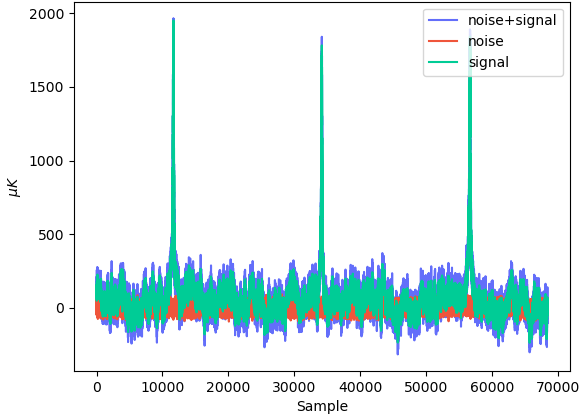
\includegraphics[width=1\linewidth]{figs/Samples_040_00274.png} 
  \caption{Time ordered data for one hour of samples for the 40 GHz channel. Both the white noise level reduced to account for the reduced number of detectors and the reduced observation time, the sky signal and the total signal are shown. The peaks correspond to scanning the galaxy plane. Units are in $\mu$K}
  \label{fig:sample_timeline}  
\end{figure} %TODO make sure this plot correspond to the same hour shown in the 1 hour plot below

Running \commanderthree\ on only one hour of scanning data, results in the top panel shown in Figure~\ref{fig:scanning_strategy}. 

\begin{figure}[t]
  \center
  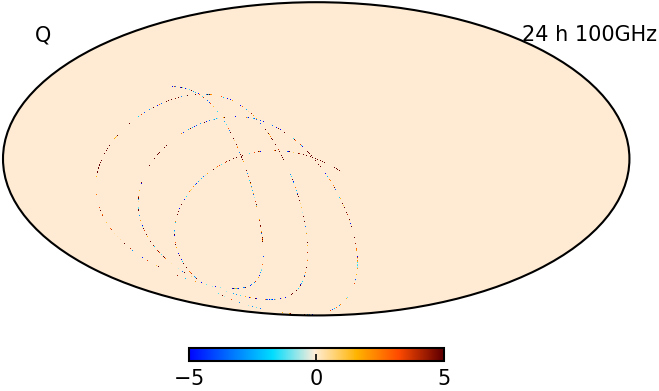
\includegraphics[width=\linewidth]{figs/tod_100a_map_c0001_k000001_Q_Stokes_w12_n512_cb_c-planck-1h.png} %TODO change to 1 hour in figure
  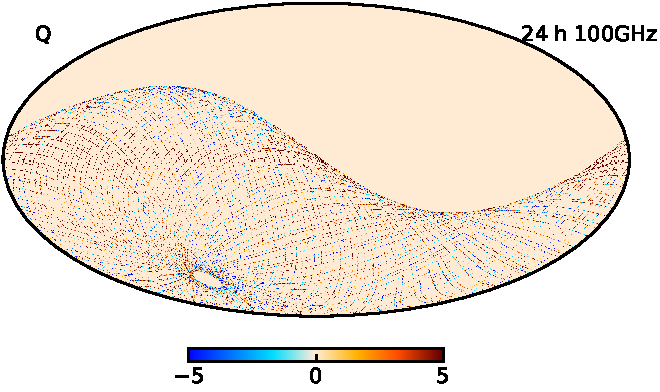
\includegraphics[width=\linewidth]{figs/tod_100a_map_c0001_k000001_Q_Stokes_w12_n512_cb_c-planck-24h.pdf}
  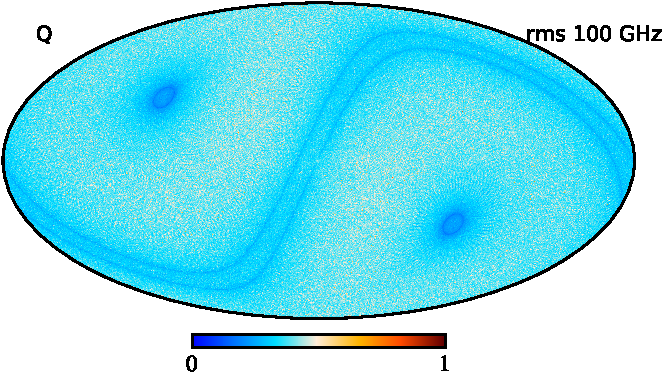
\includegraphics[width=\linewidth]{figs/tod_100a_rms_c0001_k000086_Q_Stokes_w12_n512_cb_c-planck}
  \caption{Illustration of LiteBIRDs scanning strategy. The sky map for 24 hours of scanning (top) for the 100~GHz channel, and the rms for 365 days of data (bottom) for the same channel. Both plotted in galactic coordinates.}
  \label{fig:scanning_strategy}  
\end{figure}



\subsection{Component maps}
CMB maps, foreground maps. Comparison to input
CMB map and difference input and output CMB map
foreground maps (and compare with input maps?)
\begin{itemize}
	\item Synchrotron amplitude
	\item Dust amplitude
	\item CMB
	\item probability distributions?
\end{itemize}

\begin{figure*}[t]
  \center
    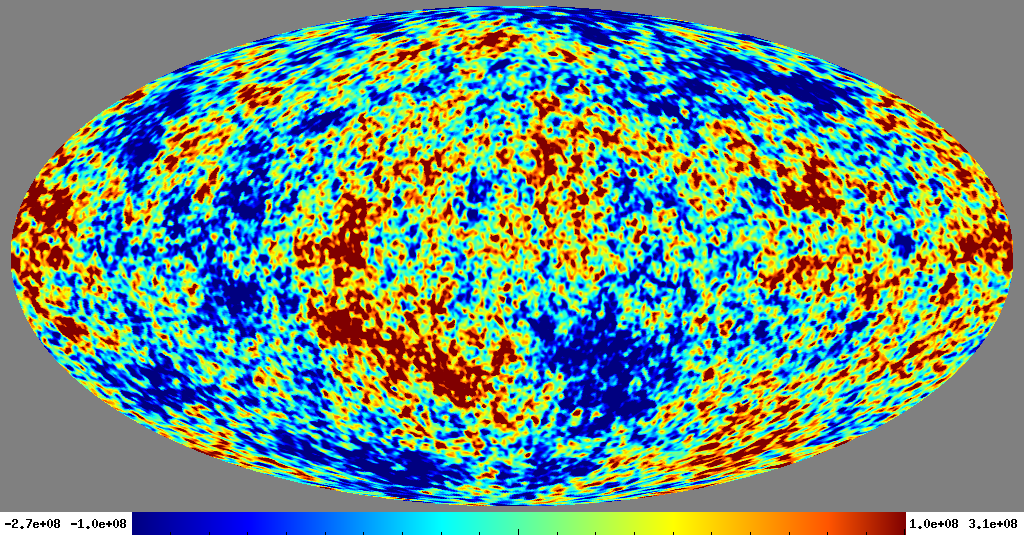
\includegraphics[width=0.33\linewidth]{figs/test_map_N256_10E5.png}
    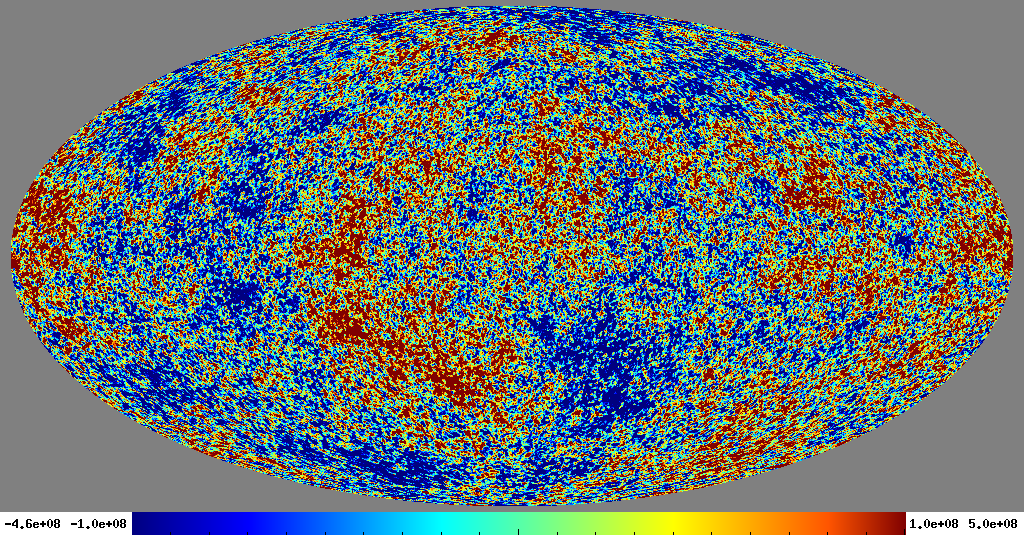
\includegraphics[width=0.33\linewidth]{figs/chains_LB_240d_40GHz_tod_040_map_c0001_k000002.png}
    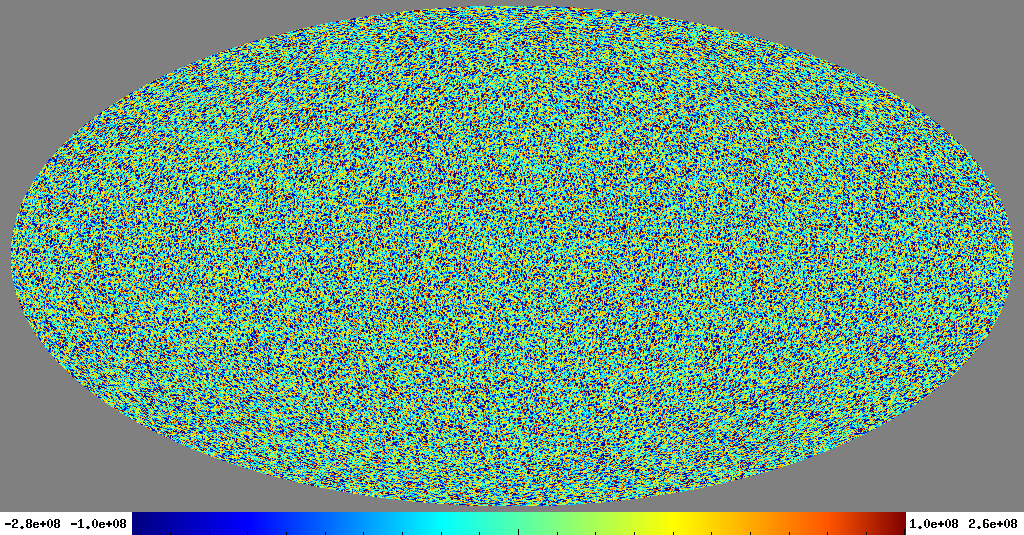
\includegraphics[width=0.33\linewidth]{figs/chains_LB_240d_40GHz_diff_todmap2_testmapE5.png}
  \caption{Input map used to generate the TOD simulation for the 40~GHz channel is shown to the left. In the middel is the resulting map generated using \commanderthree\ from 240 days of scanning. To the right is the difference between the two, with no clear patterns indicating white noise.}
  \label{fig:planck_cmb_cl}  
\end{figure*}

\subsection{r-estimation}
powerspectrum and r-estimation with Blackwell Rao estimation. 

powerspectrum?
\begin{itemize}
	\item{Of residuals}
	\item{Of run with fitting for 1/f noise and not}
	\item{Of cmb input and output and diff}
\end{itemize}
r estimation with and without removing correlated noise


\subsection{Data volume and running time}
As explained in \ref{ss:LB_sims}, only 2\%\ of the detectors and 1 out of 3 years of data collection are included in our simulations due to todays computational limitations. The data volume on disc for our simulations can be found in Table~\ref{tab:datavolume}, both before and after Huffman compression. In the same table  you can find the computational costs for running \commanderthree\ with sampling of 1/f noise, mapmaking and component separation and how much time is used to produce one sample. The analysis has been done on a computer node with 36 cores and 768 GB available memory. This gives us 240 samples/month. 

The numbers from the current simulations have been scaled up to estimate the total data volume, memory and time usage for the full LiteBIRD mission, see Table~\ref{tab:datavolume}. The total amount of data generated by LiteBIRD can be estimated to be 150 times higher than our simulations, scaling up to 4508 detectors and 3 years. We therefore estimate a total uncompressed data volume of 30~TB. According to \cite{LiteBIRD-Note-023}, the projected total amount of LiteBIRD data will be 20~TB. The increased amount of data will only effect the time used on processing the TOD, while the component separation part will not be effected since this happens in map space. We therefore estimate that we could generate 8 samples/month on 36 cores. 


\begin{table}[t] 
  \begingroup
  \newdimen\tblskip \tblskip=5pt
  \caption{
  	Estimated data volume and running time for 88 detectors and 1 year (this work) and full mission with 4508 detectors and 3 years. 
  }
  \label{tab:datavolume}
  \nointerlineskip
  \vskip -3mm
  \footnotesize
  \setbox\tablebox=\vbox{
    \newdimen\digitwidth
    \setbox0=\hbox{\rm 0}
    \digitwidth=\wd0
    \catcode`*=\active
    \def*{\kern\digitwidth}
    %
    \newdimen\signwidth
    \setbox0=\hbox{-}
    \signwidth=\wd0
    \catcode`!=\active
    \def!{\kern\signwidth}
    %
 \halign{
      \hbox to 3.5cm{#\leaderfil}\tabskip 1em&
      \hfil#\tabskip 1em&
      \hfil#\tabskip 1em&
      \hfil#\tabskip 1em&
      \hfil#\tabskip 1em&
      \hfil#\tabskip 0pt\cr
    \noalign{\doubleline}
      \omit\textsc{}\hfil&
      \omit\hfil\textsc{88 detectors}\hfil&
      \omit\hfil\textsc{4508 detectors}\hfil\cr
      \omit\textsc{}\hfil&
      \omit\hfil\textsc{1 year}\hfil&
      \omit\hfil\textsc{3 years}\hfil\cr
      \noalign{\vskip 4pt\hrule\vskip 4pt}
      \noalign{\vskip 2pt}
      \hskip 10pt Data volume			& 200 GB				& 30 TB			\cr
      \hskip 10pt Huffman compressed		& 60 GB				& 10 TB			\cr
      \hskip 10pt Memory usage			& 500 GB				& 11 TB			\cr
      \hskip 10pt Time useage			& 3 hours/sample		& 				\cr
      \omit							& 240 samples/month	& 8 samples/month	\cr} } 
  \endPlancktable \endgroup
\end{table} % TODO make more detailed based on the final run




IMOv0(v28): 365 days of TOD, 6 detectors pr channel (6*22=132 detectors), 2TB. 35\% less with IMOv1 -> 1.3TB. Scale up to 4508 detectors and 3 years: 133TB. Mission expectation from LiteBIRD is 20~TB. 




%%%%%%%%%%%%%%%%%%%%%%%%%%%%%%%


\section{Summary and conclusions}
\label{sec:Conclusions}

%1) Start with a sentence that states what the paper is about; this may be very similar to the first sentence of the abstract, and often this sentence will "close the circle" with respect to the beginning. 2) Then briefly summarize the main novel methodological features that have been introduced in the paper. 3) Then do a walk-through of the main results; one paragraph per main point. Make sure to include numerical results at this stage, whenever appropriate. Interpret the results as appropriate, and make connections to earlier results -- what is similar and what is different? 4) Then you discuss open problems and next steps. What remains to be done? What is unsolved? What is needed to make further progress? 5) If possible, end with a positive sentence.

Show r likelihood curve with fitting for correlated noise. 

Further work: Include HWP, fitting for bandpass, add systematic effects, more complicated foreground models... \commanderthree\ already support fitting for a lot of parameters not fitted for in this work. Proof of concept. 

It is however reasonable to assume that the computational power available in the early 2030s when the data from the LiteBIRD mission is ready, will be able to handle this amount of data. 11~TB. Sample more parameters. More efficient parallelization. Code development. Just estimates. 


\begin{acknowledgements}
  We thank Prof.\ Pedro Ferreira and Dr.\ Charles Lawrence for useful suggestions, comments and 
  discussions. We also thank the entire \Planck\ and \WMAP\ teams for
  invaluable support and discussions, and for their dedicated efforts
  through several decades without which this work would not be
  possible. The current work has received funding from the European
  Union’s Horizon 2020 research and innovation programme under grant
  agreement numbers 776282 (COMPET-4; \BP), 772253 (ERC;
  \textsc{bits2cosmology}), and 819478 (ERC; \textsc{Cosmoglobe}). In
  addition, the collaboration acknowledges support from ESA; ASI and
  INAF (Italy); NASA and DoE (USA); Tekes, Academy of Finland (grant
   no.\ 295113), CSC, and Magnus Ehrnrooth foundation (Finland); RCN
  (Norway; grant nos.\ 263011, 274990); and PRACE (EU).
\end{acknowledgements}


\bibliographystyle{aa}

\bibliography{../common/BP_bibliography,../common/Planck_bib,BP06_bibliography}
%citations: You should use only three types of Latex cite-tags: 1) \citet{bp01} should be used when the reference is a part of a sentence, as in "As shown by \citet{bp01}, end-to-end Gibbs sampling is cool." This will translate into "As shown by BeyondPlanck (2020), end-to-end Gibbs sampling is cool." 2) \citep{bp01} is used when the citation is not part of the sentence, but appears surrounded by parantheses, as in "End-to-end Gibbs sampling is cool \citep{bp01}" -> "End-to-end Gibbs sampling is cool (BeyondPlanck 2020)." 3) Finally, \citealp can be used for special cases when you want to do the formatting yourself, for instance if the reference appears inside a full sentence inside parantheses, as in "End-to-end Gibbs sampling is cool (as shown by \citealp{bp01})." -> "End-to-end Gibbs sampling is cool (as shown by BeyondPlanck 2020)."
%\appendix

%\section{Appendix}
%\label{app:appendix}



\end{document}
